\section{Specification and implementation of distributed systems}

\subsection{Event based component model}
Each node models a sequential program. There is a global clock
and at each tick either a node takes a one of the following step
\begin{itemize}
	\item Computation step: Perfoms computation (local) or
	sends/receives one message to/from other nodes (global)
	\item Communication step: deliver a message.
\end{itemize}
There are different models for the delivery:
\begin{enumerate}
    \item Receive 1 msg and send 1 msg (Guerraoui)
    \item At most receive 1 msg and send at most 1 msg to each neighbor (Lynch)
    \item Receive k msg and send at most 1 msg to each neighbor (Welch)
\end{enumerate}


\paragraph{ }
Each program consists of a set of \textbf{modules or component
specifications}

We study 2 main kinds of distributed systems: \textbf{communications} and
\textbf{reliable high-level services}.

\begin{table}[!ht]
    \begin{tabular}{p{0.475\linewidth}p{0.475\linewidth}}
        \toprule
        \multicolumn{1}{c}{\bf Communication} & \multicolumn{1}{c}{\bf Reliable high-level services} \\
        \toprule
        \begin{itemize}
            \item reliable broadcast
            \item causal order broadcast
            \item total order broadcast
            \item terminating reliable broadcast
        \end{itemize}
        &
        \begin{itemize}
            \item shared memory
            \item consensus
            \item atomic commit
            \item group membership
        \end{itemize} \\
        \bottomrule
    \end{tabular}
\end{table}
\FloatBarrier{}

\subsubsection{Event}
\begin{lstlisting}[mathescape]
upon event <RequestEvent, attr$_1$, attr$_2$,...> do
    // local computation
    trigger <ResponseEvent, attr$_3$, attr$_4$,...>
\end{lstlisting}

There are three main types of event: \textbf{request, indication,
confirmation}

\subsubsection{Modules}

\begin{figure}[!ht]
    \centering
    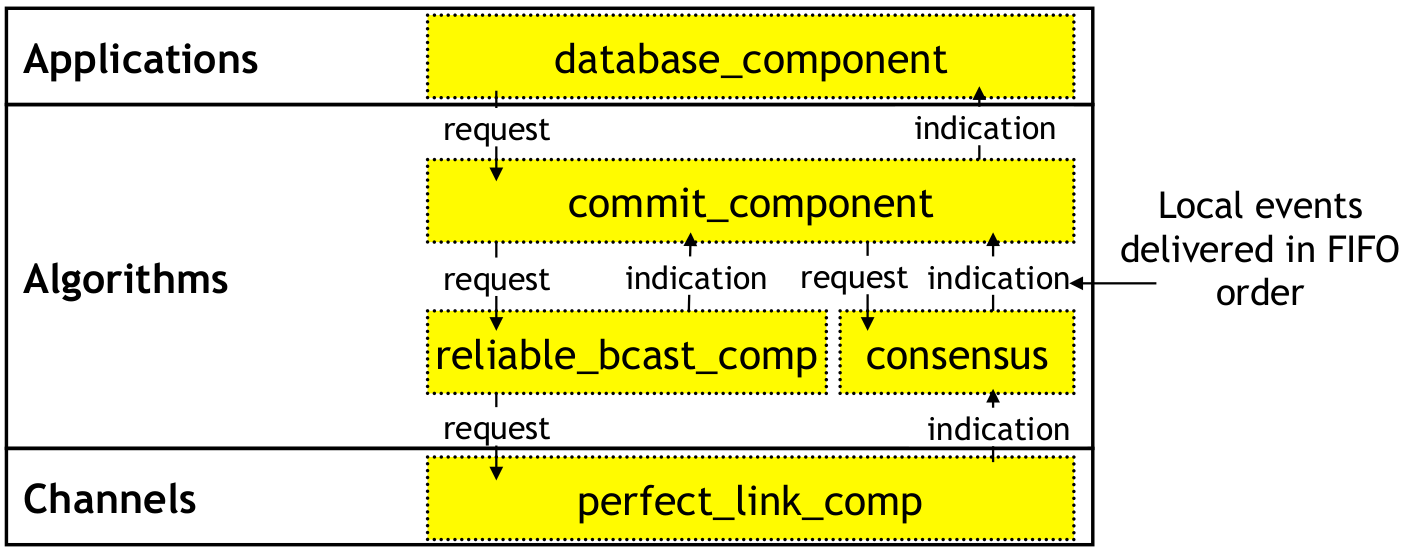
\includegraphics[width=0.6\linewidth]{img/module.png}
    \caption{Modules scheme}
\end{figure}
\FloatBarrier{}

\begin{itemize}
    \item receive instruction:  upon event $<delBcast\ |\ src, [data_1,
        data_2,\ldots] >$ do
    \item send instruction:
        trigger $<sendBcast\ |\ dest, [data_1, data_2,\ldots]>$
\end{itemize}

\begin{figure}[!ht]
    \centering
    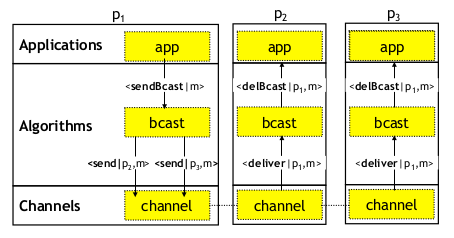
\includegraphics[width=10cm]{img/ex_broadcast.png}
    \caption{Example application uses a broadcast}
\end{figure}
\FloatBarrier{}

\subsection{Specification of a service}

Reliable applications need underlying services strong than network protocols
(such as TCP that only provides a one-to-one connection).

\begin{figure}[!ht]
    \begin{tabular}{m{0.475\linewidth}m{0.475\linewidth}}
        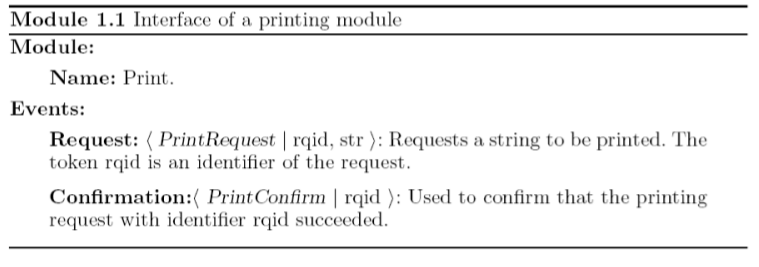
\includegraphics[width=\linewidth]{img/ex_inter1.png} &
        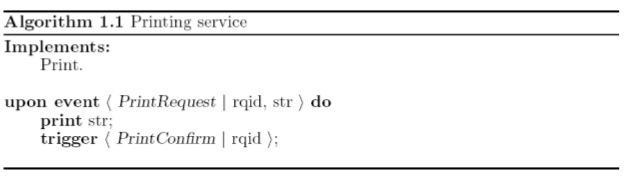
\includegraphics[width=\linewidth]{img/ex_inter2.png} \\
        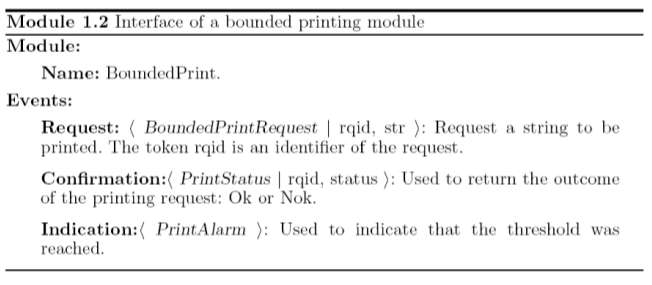
\includegraphics[width=\linewidth]{img/ex_inter3.png} &
        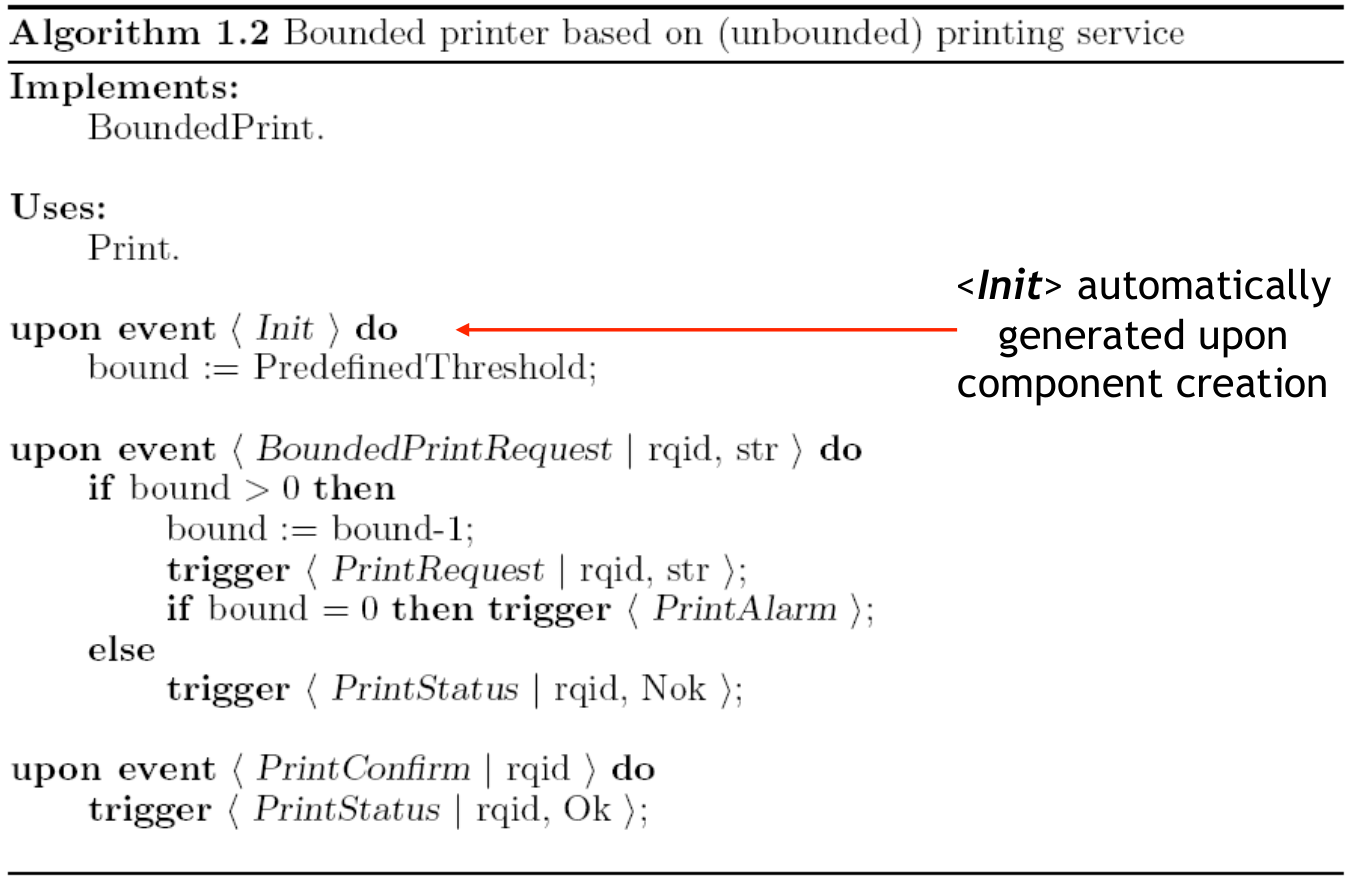
\includegraphics[width=\linewidth]{img/ex_inter4.png}
    \end{tabular}
    \caption{Interface example}
\end{figure}
\FloatBarrier{}


\subsection{Property}

A property P is a function that takes an execution and returns
true/false. (\textit{P is a predicate})

\begin{center}
    \enquote{\textit{Any [property] can be expressed as the conjunction of a
    safety property and a liveness property}}
\end{center}

\begin{itemize}
    \item \textbf{Prefix} of an execution $E$ is the first $k$ (for
        some $k>0$) configurations and events of $E$
    \item \textbf{Extension} of a prefix $P$ is any execution
        that has $P$ as a prefix

    \item \textbf{Safety}: Properties that state that something bad \textcolor{red}{never}
        happens

        \begin{figure}[!ht]
            \centering
            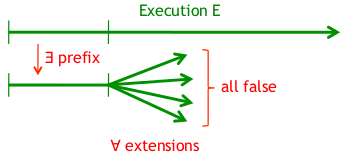
\includegraphics[width=6cm]{img/safety.png}
            \caption{Safety is false if}
        \end{figure}
        \FloatBarrier{}

        \begin{itemize}
            \item[Note:] safety can only be satisfied in infinite time and violated in
                finite time
        \end{itemize}

    \item \textbf{Liveness}: Properties that state that something good
        \textcolor{red}{eventually} happens

        \begin{figure}[!ht]
            \centering
            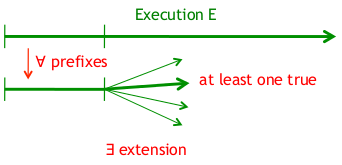
\includegraphics[width=6cm]{img/liveness.png}
            \caption{Liveness is true if}
        \end{figure}
        \FloatBarrier{}

        \begin{itemize}
            \item[Note:] liveness can only be satisfied in finite time and violated in
                infinite time
        \end{itemize}
\end{itemize}


\subsection{Failure}

\subsubsection{Node}

Nodes that don’t fail in an execution are
correct. There are different way of failure:

\begin{itemize}
    \item \textbf{Crash-stop}: stops taking steps, stops sending/receiving msg

        \begin{itemize}
            \item[$\to$] Cannot recover this failure
        \end{itemize}

    \item \textbf{Omissions}: send (resp. receive) ommission. Formally, an
        event removing element from outbuf[i] (resp. inbuf[i])

    \item \textbf{Crash-recovery}: stops taking steps but receiving and
        sending msg.

        \begin{itemize}
            \item[$\to$] We can recover after crashing with special $<Recovery>$ event
                autmatically generated.

                In practice, restarting in initial recovery state or on
                the save state if we make some (expensive) storage on
                permanent storage device.
        \end{itemize}

        A node is faulty in an execution if it crashes and never
        recovers or crashes/recovers infinitely.

        A correct node may crash and recover.

    \item \textbf{Byzantine}: sending messages/updating its state
        not specified by its algorithm.

        \textit{may behave maliciously, attacking the system}

\end{itemize}

\begin{figure}[!ht]
    \begin{tabular}{m{8cm}m{8cm}}
        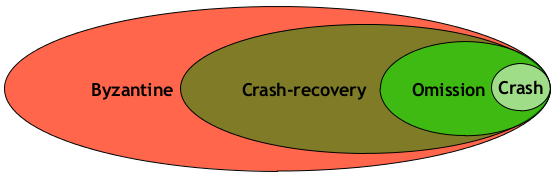
\includegraphics[width=8cm]{img/fault-tolerance.png}
        &
        \begin{itemize}
            \item If node use stable storage: crash-recovery = omission
            \item If node use volatile storage: crash-recovery extend omission
                with amnesia
        \end{itemize}
    \end{tabular}

    \caption{Fault tolerance}
\end{figure}
\FloatBarrier{}

\subsubsection{Channel}

\begin{itemize}
    \item \textbf{Fair-loss links}: Channel delivers any message sent
        with non-zero probability

        \begin{lstlisting}[caption= Fair loss link interface]
Request: <flp2pSend | dest, m>
Indication: <flp2pDeliver | src, m>
        \end{lstlisting}

        \begin{enumerate}
            \item FL1. \textbf{Fair-loss}: If $m$ is sent infinitely
                often by $p_i$
                to $p_j$, and neither crash, then $m$ is delivered infinitely
                often by $p_j$
            \item FL2. \textbf{Finite duplication}: If a $m$ is sent a finite
                number of times by $p_i$ to $p_j$, then it is delivered a
                finite number of times by $p_j$
            \item FL3. \textbf{No creation}: No message is delivered unless it
                was sent
        \end{enumerate}

    \item \textbf{Stubborn links}: Channel delivers any message sent
        infinitely many times (to implement it, we use fair-loss link, each node
        stores the messages sent and periodically resends them).

        \lstinputlisting[caption={Stubborn link interface}, mathescape, captionpos=b]{listings/stubborn_link_interface.erl}

        \begin{enumerate}
            \item[SL1] \textbf{Stubborn delivery}: if a node $p_i$ sends a
                message $m$ to a correct node $p_j$, and $p_i$ does not
                crash, then $p_j$ delivers $m$ an infinite number of
                times

            \item[SL2] \textbf{No creation}: if a message $m$ is delivered by
                some node $p_j$, then $m$ was previously sent by
                some node $p_i$
        \end{enumerate}

    \item \textbf{Perfect links}: Channel that delivers any message
        sent exactly once (keep a set of delivered msg)

        \begin{lstlisting}[caption=Perfect links, mathescape, captionpos=b]
upon event <Init> do
    delivered := $\emptyset$

upon event <pp2pDeliver | dst, m> do
    trigger <sp2pSend | dst, m>

upon event <sp2pDeliver | src, m> do
    if m $\notin$ delivered then
        delivered := delivered $\cup$ {m}
        trigger <pp2pDeliver | src, m>
\end{lstlisting}


        \begin{enumerate}
            \item[PL1] \textbf{Reliable delivery} (liveness):
                If neither $p_i$ nor $p_j$ crashes, then every message sent
                by $p_i$ to $p_j$ is eventually delivered by $p_j$

            \item[PL2] \textbf{No duplication} (safety): Every message is delivered
                at most once

            \item[PL3] \textbf{No creation} (safety): No message is delivered unless it was
                sent
        \end{enumerate}

\end{itemize}

\subsection{Timing assumptions}

Different processing speeds of nodes and different speeds of messages.

\subsubsection{Local vs Global}
\begin{itemize}
    \item Local (one node = State)
        \begin{itemize}
            \item Atomic
            \item Deterministic
        \end{itemize}
    \item Global (many nodes = Configuration)
        \begin{itemize}
            \item Non-atomic (because piece of code in many nodes)
            \item Non deterministic (because of the network and message re-ordering)
        \end{itemize}
\end{itemize}


\subsubsection{Synchronous vs Asynchronous}
\begin{itemize}
    \item Asynchronous: No timing assumption on nodes and channels.

        \begin{itemize}
           \item Lamport clocks (or vector clocks) to observe causality.
           \item Total order not observable
       \end{itemize}

       Internet is asynchronous!

    \item Synchronous: Use round to synchronize (like clock) and this
        is used to detect failure

    \item Partial synchonous: asynchronous system which eventually
        becomes synchronous.

        \textit{It’s just a way to formalize the following: Your
            algorithm will have a long enough time
            window, where everything behaves nicely
        (synchrony), so that it can achieve its goal}
\end{itemize}


\begin{figure}[!ht]
    \centering
    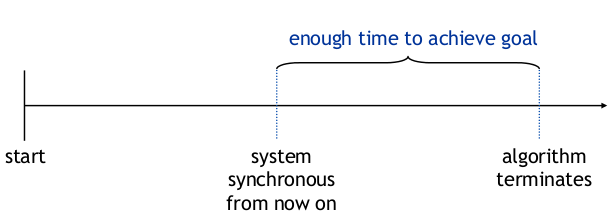
\includegraphics[width=8cm]{img/partialsynchronous.png}
    \caption{Partial synchony}
\end{figure}
\FloatBarrier{}
